\chapter{Benchmarks and evaluation}
\section*{\fshark{} generated Futhark compared to original Futhark code}

Appendices show 
\section*{The \texttt{LocVolCalib} benchmark}
small.in:
FShark (openCL) took 211882 microseconds.
Average invokation (fshark non openCL) time was 81194767 microseconds.
Native took 438 929 311 microseconds.

\begin{figure}
    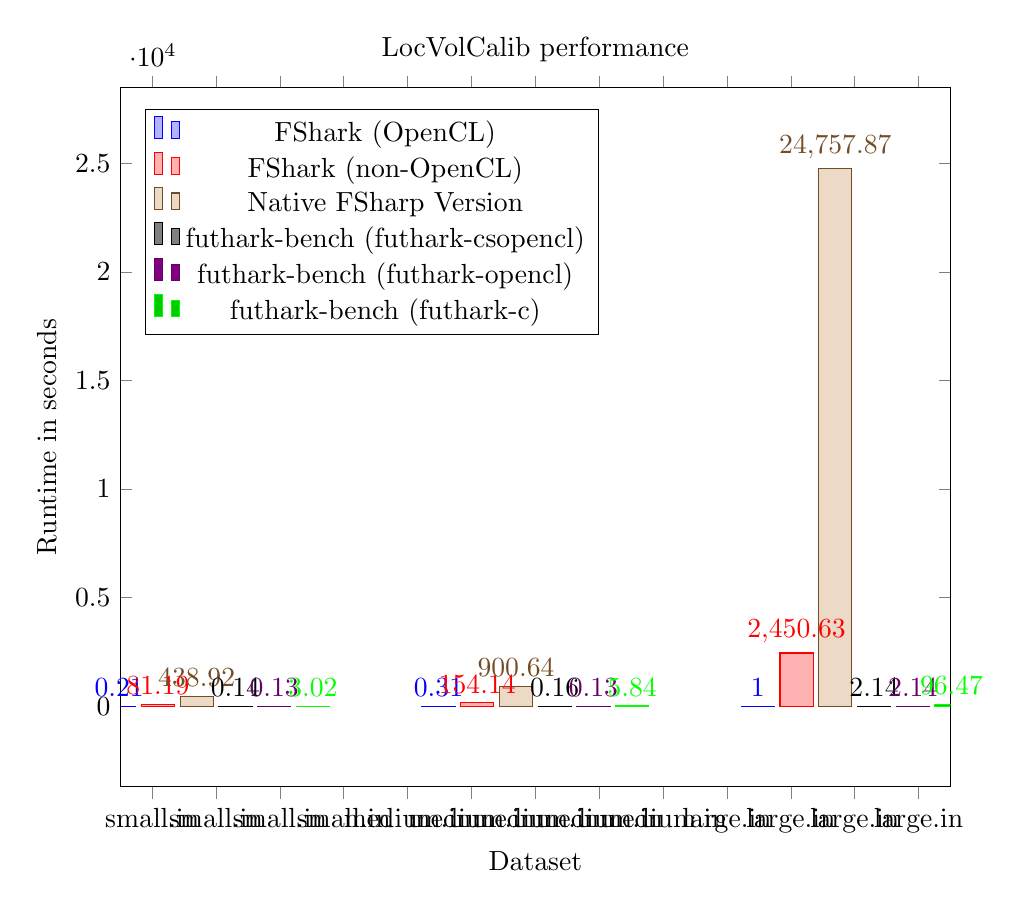
\begin{tikzpicture}
      \begin{axis}[
        title={LocVolCalib performance},
        xlabel={Dataset},
        ylabel={Runtime in seconds},
        width=1\textwidth,
        %height=0.5,
        symbolic x coords={small.in,medium.in,large.in},
        bar width=9pt,
        enlargelimits=0.15,
        ybar=2pt,% configures ‘bar shift’
        bar width=12pt,
        nodes near coords,
        legend style={legend pos=north west}
      ]
      \addplot plot coordinates {(small.in, 0.21 ) (medium.in, 0.31 ) (large.in, 0.9999 )};
      \addplot plot coordinates {(small.in, 81.19 ) (medium.in, 154.14 ) (large.in, 2450.63 )};
      \addplot plot coordinates {(small.in, 438.92 ) (medium.in, 900.64 ) (large.in, 24757.87 )};
      \addplot plot coordinates {(small.in, 0.14 ) (medium.in, 0.16 ) (large.in, 2.14 )};
      \addplot plot coordinates {(small.in, 0.13 ) (medium.in, 0.13 ) (large.in, 2.14 )};
      \addplot plot coordinates {(small.in, 3.02 ) (medium.in, 5.84 ) (large.in, 96.47 )};

      \legend{FShark (OpenCL), FShark (non-OpenCL), Native FSharp Version, futhark-bench (futhark-csopencl), futhark-bench (futhark-opencl), futhark-bench (futhark-c)}
      \end{axis}
    \end{tikzpicture}
    \caption{Comparison between Python and Futhark performance for simple model}
    \label{fig:line-graph}
\end{figure}

medium.in:
(Fshark opencl)invokation time was 310833 microseconds
Fshark nonopencl Average invokation time was 154 141 321 ms
Native took 900 643005 microseconds.

large.in:

fshark with opencl Memory Allocation Error
fshark sans opencl 2450 637 053 microseconds
Native took 24757 874 577 microseconds.


for all three datasets
%% master ●  futhark-bench --compiler=futhark-csopencl LocVolCalib.fut 
%%Compiling LocVolCalib.fut...
%%Results for LocVolCalib.fut:
%%dataset LocVolCalib-data/small.in:   143141.00us (avg. of 10 runs; RSD: 0.02)
%%dataset LocVolCalib-data/medium.in:  163246.30us (avg. of 10 runs; RSD: 0.00)
%%dataset LocVolCalib-data/large.in:  2143760.90us (avg. of 10 runs; RSD: 0.00)
%%
%% master ●  futhark-bench --compiler=futhark-opencl LocVolCalib.fut 
%%Compiling LocVolCalib.fut...
%%Results for LocVolCalib.fut:
%%dataset LocVolCalib-data/small.in:   134473.30us (avg. of 10 runs; RSD: 0.02)
%%dataset LocVolCalib-data/medium.in:  134796.20us (avg. of 10 runs; RSD: 0.01)
%%dataset LocVolCalib-data/large.in:  1924412.20us (avg. of 10 runs; RSD: 0.01)

%% master ●  futhark-bench --compiler=futhark-c LocVolCalib.fut     
%%Compiling LocVolCalib.fut...
%%Results for LocVolCalib.fut:
%%dataset LocVolCalib-data/small.in:  3 020588.60us (avg. of 10 runs; RSD: 0.01)
%%dataset LocVolCalib-data/medium.in: 5 842482.00us (avg. of 10 runs; RSD: 0.01)
%%dataset LocVolCalib-data/large.in:  96 476520.00us (avg. of 10 runs; RSD: 0.00)
%%


\section*{The \texttt{nbody} benchmark}

for all three datasets


\subsection*{Specifications for benchmark}
We have run the benchmarks on a system with these attributes:
\begin{itemize}
\item CPU: 4 cores of Intel Core i5-6500 at 3.20GHz
  \begin{itemize}
  \item L1 cache: 128 KiB 
  \item L2 cache: 1024 KiB 
  \item L3 cache: 6144 KiB 
  \end{itemize}
\item GPU: GeForce GTX 970
\end{itemize}


Introduction for the two benchmarks LocVolCalib and nbody



why are they faster in general



%%% Local Variables:
%%% mode: latex
%%% TeX-master: "../thesis"
%%% End: